% radon veto, v1.0

\chapter{The radon veto}~\label{ch:rnveto}

\paragraph{Abstract} While the tracking of individual ions in a detector is not a novel concept, no one has yet shown its effectiveness or feasibility when also coupled with the movement of the bulk fluid through which the ions travel. In this chapter we cover the so-called ``radon veto'', which proposes to follow atoms of the uranium decay chain throughout the XENON1T detector and remove the corresponding \Pb~events from the analysis. This has the potential to significantly boost the sensitivity of the experiment at a marginal cost of exposure.

If it is possible to follow atoms of \Po~around the detector, the next step is to follow atoms further down the decay chain. If \Pb~atoms can be followed and their decays identified, these events can be removed from the analysis. As \Pb~is the dominant background source in the dark matter region of interest~\cite{Aprile:2015uzo}, this has the possibility to significantly boost the sensitivity of the experiment at a marginal cost in exposure. We exploit the fact that because \Pb~is part of a decay chain, the times and positions of its decays have physical significance to the atoms surrounding it.

We will begin with a brief review of the relevant portion of the decay chain of primordial uranium, as shown in Figure~\ref{fig:useries}. \Pb~decays to the ground state of $^{214}$Bi with a branching ratio of $11.0\%$, and a fraction of these decays lie in the dark matter signal region of interest. This is the primary cause of background in this energy range~\cite{Aprile:2015uzo}.

\begin{figure}[htb]
\centering
    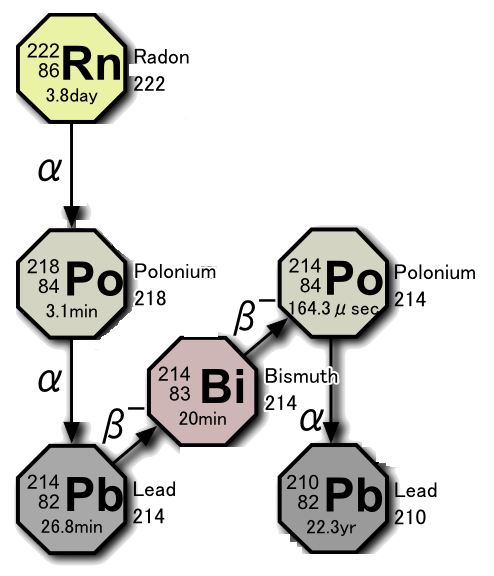
\includegraphics[width=\textwidth]{figures/rnveto/uranium_series}
    \caption{\todo{PLACEHOLDER IMAGE} A section of the decay chain of primordial ${}^{238}$U. Atoms of \Rn~emanate out of impurities in the metals used in detector construction and mix throughout the xenon volume. Low-energy decays of \Pb~that decay directly to the ground state of $^{214}$Bi are the leading cause of background in the dark matter ROI.}\label{fig:useries}
\end{figure}

\section{Technique overview}

While there is nothing about a \Pb~event that is easily identifiable, its parent isotopes (\Rn, \Po) and daughter (\BiPo) can be identified with relative ease using alpha spectroscopy or the BiPo timing structure~\cite{Aprile:2017fhu}. This allows us to bookend the \Pb~event with events that are more easily identified. With this information, an algorithm resembling one for track reconstruction can be employed to improve the confidence with which \Pb~events are tagged by identifying the decays of the parents and daughtber and looking for the convection streamlines that connect them. The \Pb~decay must happen somewhere on the streamline between the \Po~and \BiPo~decays. A stylized representation of this is shown in Figure~\ref{fig:rnveto_schematic} where displacement due to convection is normalized out.

\begin{figure}[htb]
\centering
    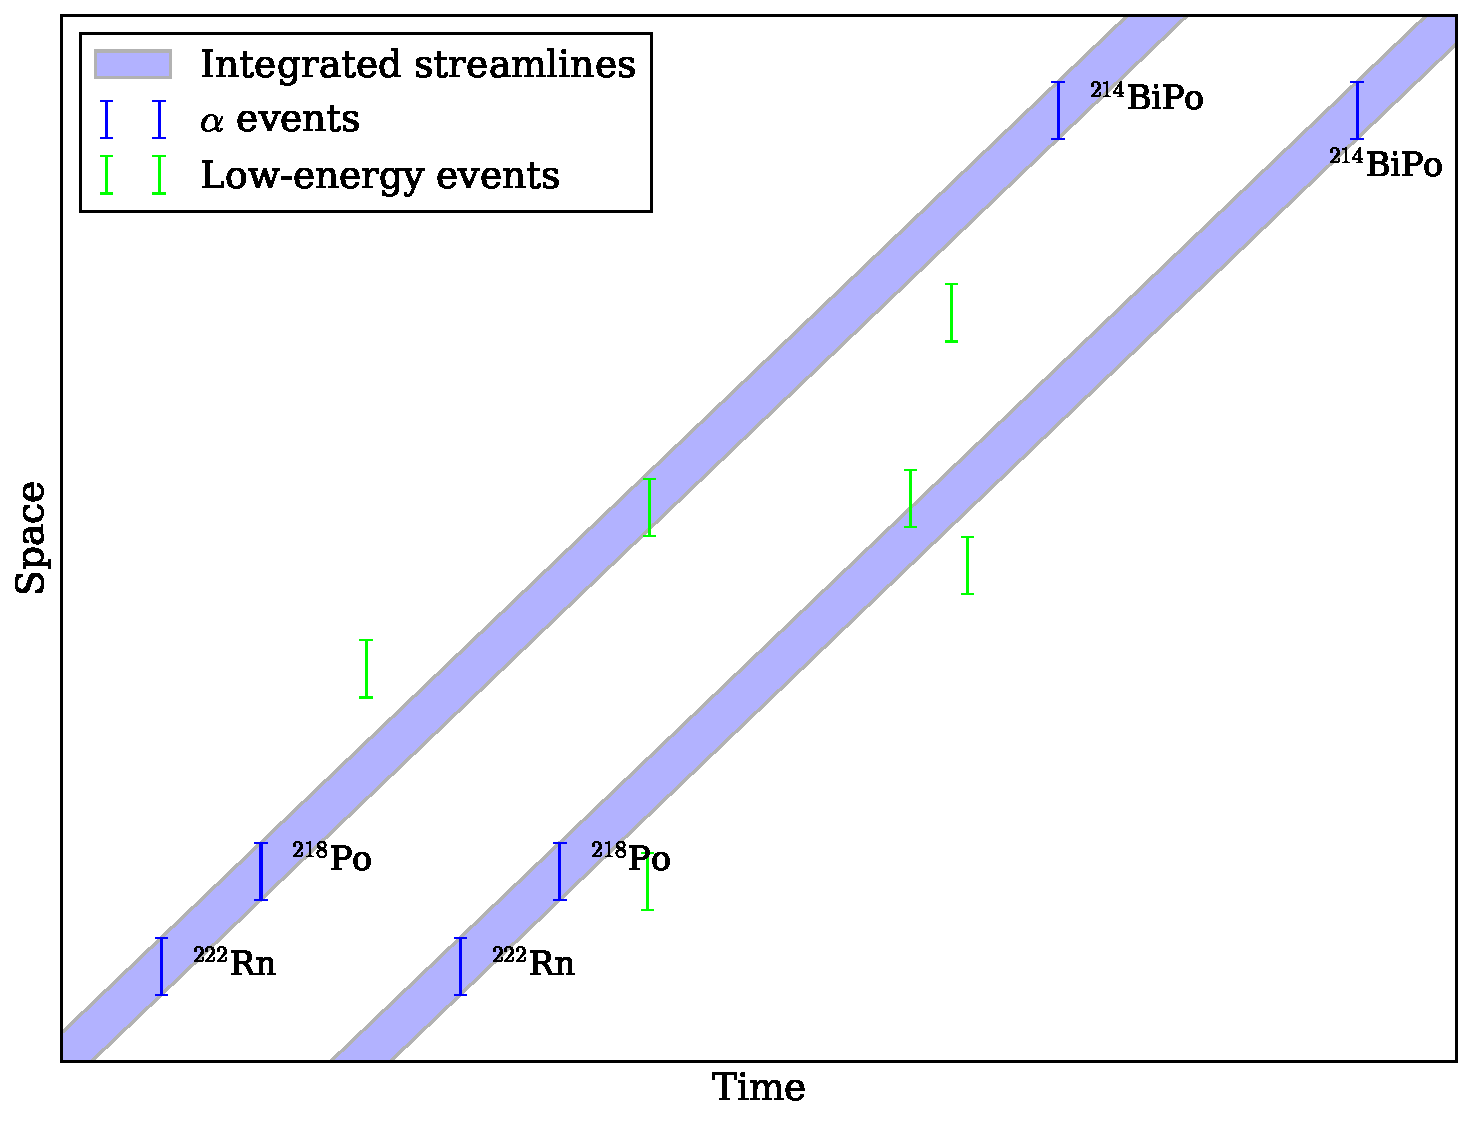
\includegraphics[width=\textwidth]{figures/rnveto/rnveto_schematic}
    \caption{A simple schematic of how the radon veto works. Low-energy events (in green) due to \Pb~can be identified because they occur on streamlines (shaded regions) connecting \Rn, \Po, and \BiPo~events (in blue), while low-energy events due to other background sources occur at random.}\label{fig:rnveto_schematic}
\end{figure}

\section{Convection-agnostic approach}

To demonstrate a proof of this concept, we employ a convection-agnostic approach. In this method, a sphere is placed around every \Po~or \BiPo~event. Regardless of the size of the sphere or how long one watches it, some fraction of \Pb~decays will occur within it. The size of the sphere can be related to the length of observation time by the average speed of convection, and the observation time can be chosen by a simple optimization to maximize the potential background reduction while minimizing the overall exposure cost.

The principle background to this Big Sphere method is that of false positives from random coincidence. This can be very easily quantified through a simple Monte Carlo by placing spheres at random locations and random times within the detector, monitoring the sphere for the specified duration, and counting the number of times a low-energy event is observed. This can then be repeated using locations and timestamps of \Po~or \BiPo~events rather than at random. This allows for the clear quantization of the significant of the result. This was applied to science run 0, with results shown in Figure~\ref{fig:bs_sr0}.

\begin{figure}[htb]
\centering
    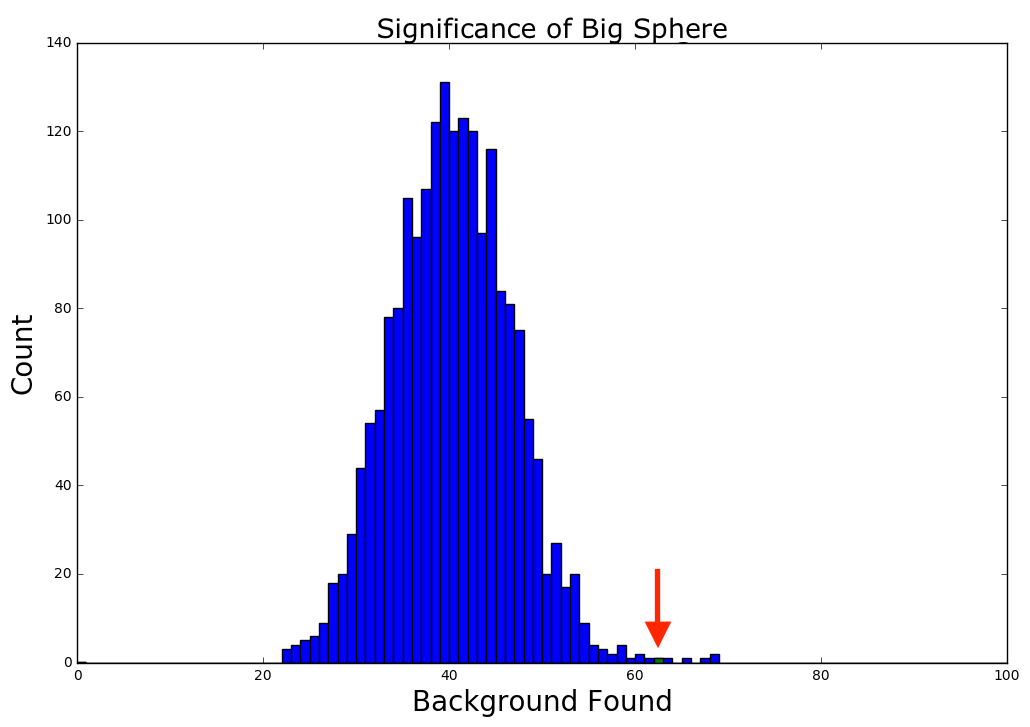
\includegraphics[width=\textwidth]{figures/rnveto/BigSphere}
    \caption{\todo{PLACEHOLDER IMAGE} (Top) The results for the convection-agnostic Big Sphere method for science run 0. The background from false positives is well-modeled with a binomial distribution. The number of events found by searching near \Po~and \BiPo~is \todo{XX}. This has a p-value of \todo{YY}, indicating a significant result. Of these events identified, \todo{XX} are in the dark matter signal ROI (bottom)}\label{fig:bs_sr0}
\end{figure}

\section{Cloud approach}

The Big Sphere method has a number of limitations. Looking in all directions rather than just along the convection streamlines wastes a large amount of exposure, and in cases where multiple low-energy events are observed within the sphere it is impossible to proceed. At most one can be due to \Pb, yet without additional information it is impossible to determine which. This additional information can be found from convection. If an event is on fluid streamlines originating from the \Po~decay vertex or converging to the \BiPo~vertex, it is more likely to be \Pb~than if it occurred far from those streamlines or on otherwise impossible paths.

The computational cost of following these streamlines is non-trivial. It involves a numerical integration of a vector field, and doing this multiple times. Each \Rn~atom can potentially produce a low-energy \Pb~event, so streamlines around every \Rn~must be followed. At a decay rate of $\approx 2500\1{day^{-1}}$, a tonne-year of exposure will contain nearly $500\,000$ total \Rn~events. Streamlines from each of these events must be integrated for (on average) one hour, at sufficiently small timesteps to minimize integration errors.

\section{Diffusion-limited case}

The dominant uncertainties to the radon veto stem from the lack of complete knowledge of the convection pattern. However, we can explore the possibilities of the technique should a perfect understanding of convection be obtained. In this limit, the dominant uncertainties are from position reconstruction and diffusion.

\subsection{Diffusion effects}

When an event happens, we reconstruct its interaction vertex with a uncertainty of $5\1{mm}$ in r and $1\1{mm}$ in z. For reasons we will discuss shortly, we will take 2 sigma and double these. Thus, we assume this event happens somewhere in a cylinder of volume $\approx 630\1{mm^3}$. This cell will follow the convection lines through the volume, growing in time due to diffusion. We'll need a few values here:
\begin{itemize}
    \item $r_0 = 10\1{mm}$
    \item $h_0 = 2\1{mm}$
    \item Cell volume: $V(t=0) = \pi r_0^2h_0 = 630\1{mm^3}$
    \item Diffusion constant: $D = \frac{k_BT}{6\pi\eta r} = 1.7\times10^{-3}\1{mm^2/s}$
\end{itemize}

We find the diffusion constant via the Stokes-Einstein relation for a spherical particle diffusing through a fluid at low Reynolds number~\cite{Sutherland:1905,Einstein:1905,Smoluchowski:1906}. $\eta$ is the viscosity ($0.5\1{mPa s}$~\cite{Legros:1965}) and $r$ is the radius of the particle in question (taken as $0.15\1{nm}$). The displacement of the atom from its initial location will be roughly given by $\Delta s = \sqrt{\pi Dt}$, and the increase in volume can be found by adding $\sqrt{\pi Dt}$ to both r and z. Thus

\begin{equation}
V(t) = \pi(r_0 + \sqrt{\pi Dt})^2(h_0 + \sqrt{\pi Dt})
\end{equation}

Starting from a decay of \Po, in one half-life of its daughtber ($\sim$30 min) the cell volume will increase by $2.1\1{cm^3}$ to a total of $2.75\1{cm^3}$. If we see an ER event in this volume in the energy range we would expect from a \Pb~decay, we can cut this event (and stop following that cell as it is no longer a potential background event).

\subsection{Total vetoed volume}

The next value to calculate is what fraction of the active region we can follow. For that we need to calculate how many atoms we need to follow at any one time. As calculated above, we find that on average the detector will contain these populations:
\begin{itemize}
    \item $N_{Rn} = 13\,300$
    \item $N_{Po} = 7.5$
    \item $N_{Pb} = 66$
    \item $N_{Bi} = 48$
\end{itemize}

Atoms further down the decay chain will have slightly reduced populations due to plateout and cathode cleaning, but these values are upper limits. The probability that we must still follow the atom in that volume is $P(t) = \exp -\lambda t$ (if the atom decays, we no longer need to follow it), and the expression for the cell volume is given above.

If we wish to reduce the contribution of \Pb~to the low-energy background to the point where it becomes equivalent or subdominant to the other sources of ER background, this requires that we veto about 90\% of all low-energy lead events. This means we have to follow a cell for 3 or 4 half-lives, and for this reason we took 2 sigma of the position uncertainty (giving us 95\% of the atoms). The results change very little if we follow the atom around for an infinite number of half-lives, so we will integrate over all time, not just the few half-lives we need, which results in convenient closed-form expressions.

To find the average cell volume we integrate the volume $V(t)$ with the probability density $P(t) = \lambda \exp -\lambda t$ to get

\begin{equation}
\left< V \right> = \int_0^{\infty} \dd t\,V(t) P(t) = \int_0^{\infty} \dd t\,\pi(r_0 + \sqrt{\pi Dt})^2(h_0 + \sqrt{\pi Dt})\lambda\exp -\lambda t
\end{equation}

The result is

\begin{equation}
\left< V \right> = V_0 + a\sqrt{\chi} + b\chi + c\chi^{3/2}
\end{equation}

where
\begin{itemize}
    \item $\chi = \frac{D}{\lambda}$ (units of $\n{mm^2}$)
    \item $a = \frac{\pi^{2}}{2} (r_0^2+2 r_0 h_0) = 690\1{mm^2}$
    \item $b = \pi^2 (2r_0 + h_0) = 220\1{mm}$
    \item $c = \frac{3}{4} \pi^{3}$
\end{itemize}

For \Pb, $\chi = 4\1{mm^2}$, so $\Delta V = 2.5\1{cm^3}$ or the total volume we must follow per atom is $V_0 + \Delta V = 3.1\1{cm^3}$. Given the average number of \Pb~atoms we expect to have, this will be a total vetoed volume of $200\1{cm^3}$. This is only $10^{-4}$ of the total active volume, and vetoing these volumes has a negligible cost in exposure. We can also calculate the total volumes to track for the parent and daughtber isotopes, but this is only for tagging purposes as we have no need to veto events that aren't \Pb.

If we take a pessimistic approach where we follow each cell for four half-lives (regardless of whether or not the atom in it decays), we find a total vetoed volume of $V(4T_{1/2}) = 300\1{cm^3}$ \todo{CHECK}. Thus, the $200\1{cm^3}$ value is reasonable from this point as well.

\subsection{Effect of the drift field}

We expect the drift field to cause the motion of any charged daughtber products to diverge from that of the xenon bulk. This effect can be simulated, but measuring the charge on the daughter ion will be difficult, and this uncertainty reduces the effectiveness of any simulation involving this aspect. In effect it will cause a net downward motion, which will move the ion into other streamlines (or potentially plate onto the cathode). Additionally, as we inject the liquid below the cathode, ions in the liquid will probably have difficulty passing through the cathode mesh and into the drift region.

EXO-200 found~\cite{Albert:2015vma} radon daughtber ion drift speeds of $\sim 1\1{mm/s}$ at a drift field of $350\1{V/cm}$, with ion neutralization time proportional to the electron lifetime. Additionally, they measured the fraction of radon chain decays that leave the daughtber in an ionized state. In XENON100 the ion drift was a small correction to the $\sim 8\1{mm/s}$ flow speed.
